\documentclass[sigconf,nonacm]{acmart}
%% \BibTeX command to typeset BibTeX logo in the docs
\AtBeginDocument{%
  \providecommand\BibTeX{{%
    \normalfont B\kern-0.5em{\scshape i\kern-0.25em b}\kern-0.8em\TeX}}}

\begin{document}

\title{CS145 Team 22 Midterm Report}

\author{Hamlin Liu}
\affiliation{%
  \institution{UCLA, 805103522}
  }
\email{hamlin.liu@gmail.com}
\author{Shriniket Buche}
\affiliation{%
  \institution{UCLA, 305088562}
  }
\email{shriniketbuche@gmail.com}
\author{Juan Estrada}
\affiliation{%
  \institution{UCLA, 105347991}
  }
\email{juanestrada@ucla.edu}
\author{Yash Lala}
\affiliation{%
  \institution{UCLA, 905159212}
  }
\email{yashlala@gmail.com}
\author{Justin Yi}
\affiliation{%
  \institution{UCLA, 905123893}
  }
\email{joostinyi00@gmail.com}
\renewcommand{\shortauthors}{Team 22}

\begin{abstract}

COVID-19, the theme of our CS 145 project, has been classified as a worldwide
pandemic. The rate of its spread is a complex function of local social
distancing, government policy, climate, and temporal factors, just to name a
few. Detailed analysis of all of these contributory causes is not humanly
possible. However, we can build reasonably accurate disease models by using the
Data Mining techniques taught in CS 145. This report documents our team’s
efforts towards analyzing COVID-related data in over the majority of the year
to allow for predictive forecasting. 

We catalogue our problem at hand, initial data preprocessing, exploratory
efforts toward modeling our problem, and our future predictions as we construct
a model capable of predicting fatalities caused by COVID-19, namely through the
use of a hybrid linear, exponential, and autoregressive models. 

\end{abstract}

\maketitle

\section{Introduction}

\subsection{Background}

The increasing spread of COVID-19 poses a substantial impact on the status of
global health and economy, and having accurate forecasts of the number of
affected can better inform local and national governmental bodies to make
decisions to promote public health and safety and keeping the economy afloat.
As we position to tackle this problem, we inspect our the data we have on hand:
we were given reports of various state-wide features of the COVID-19 infection
profile from as early as April, we are specifically interested in the ability
to predict the number of cases and deaths for a particular state.

\subsection{Related Work}
Notable advances in this domain are noted. Nesteruk \cite{Nesteruk} models the
progression of the pandemic using the Susceptible, Infected, Removed (SIR)
paradigm, which aims to find correlated differential equations to model flow
between different partitions of the studied population. 
\cite{EJMO} uses more direct curve estimation methods such as Holt and ARIMA on
the number of coronavirus cases in of interest, (e.g. Germany, Japan, Turkey,
the UK, etc.). These models predict the actual number of coronavirus cases to a
high degree of statistical significance. 
Others have applied novel iterative methods based on cubic spline interpolation
and Euler's methods towards predicting the spread of the virus \cite{APPADU2020}.

\section{Data Preprocessing}
Now moving on to actually wrangling the data for processing and straightforward
input to our prospective models, we first needed to examine the existing data
to analyze where help was needed. 

Upon inspection of data types, it is noted
that much of our data is numerical, bar the categorical and ordinal columns of
Province\_State and Date, respectively. We chose to convert the date from a
string type to datetime object type, to ease future parsing. Using our
contextual knowledge of our problem space, we chose to address the modeling
problem from an individual Province\_State perspective, i.e. we grouped our
data by the Province\_State field. From here on, we will refer to this
“Province\_State” field simply as the “state”. As a group we went back and
forth on whether having so many models would result in higher variance due to
the increased complexity of the model, but we decided on separate models due to
different restrictions imposed by policy makers on interstate travel and the
general thought that most people would be sheltering in place, and thus would
not travel between states.

\subsection{Round 1}
Our initial imputation strategy went as follows: We examined each state’s
numeric data column by column. If null values comprised more than 70\% of the
total data in the column, we dropped the entire column; otherwise, we replaced
all null values with the median value in our column. After noting that this
approach led to “plateaus” in our data, we tried linearly interpolating the
values in each column. This approach produces more organic data in each column,
but fails to impute data at the beginning of a time series (due to having no
“base point” to interpolate off of). Because our current models treat every
column separately, we don’t anticipate that this will cause issues; we can drop
NaN values to create new “columns” that are perfectly interpolated, but start
at a later date.  

After interpolating the data, we normalized it to zero mean unit variance. At
this time, we are still considering whether to normalize the data globally or
within a single column. Intuition would suggest that a column-wise approach
would be best. We performed these steps before really definitively knowing what
sort of modeling approach we were interested in taking, as we will discuss,
this normalization was ultimately unused, since we were working with more
direct regression methods that did not benefit from this scaling, but did drop
the null data points.

\subsection{Round 2}
At this point in time, we decided on scrapping our explorations of different
forecasting implementations to be detailed below, and focused on univariate
feature fitting methodologies for forecasting a function to fit the observed
count of confirmed cases and deaths, namely that of Holt-Winters exponential
smoothing, ARIMA for forecasting, and a simple linear model from a particular
day offset. As a result, we did not normalize our data and just allowed the
models to drop the null values from the training dataset.

However, for this round, we needed to obtain new data since our round 2 dataset
only went up to November 22nd. To do this, we created a simple Python web scraper that 
would download the new daily files from the Johns Hopkins University CSSE COVID-19 
dataset \cite{JHUdataset} which updates everyday with a new comma-separated-values file.
Thus we were able to obtain the confirmed COVID-19 case and death count of each state
within the US up to December 5th, 2020.


\section{Problem Definition}
We are given a dataset of various COVID-related features (eg. testing rate,
deaths, confirmed cases), as well as a dataset of various movement-related data
(traffic flow into and out of two states, respectively). 
We must train a machine learning model on this data, and use it to predict the
future rates of death and confirmed cases of COVID-19. 

The competition is divided into 2 rounds. The first round was to predict the
case and death count of each of the 50 states from September 1st to September
26th given any COVID-19 related data from April 12th to August 31st. The second
round was to predict the case and death count of each of the 50 states during
the winter holiday surge, specifically from December 7th to December 12th. 
For
the second round, the method can train on any any COVID-19 related data from
April 12th to December 6th. 

Our model's accuracy will be gauged via the Mean Absolute Percentage Error
(MAPE) metric, which is defined as the average of the absolute error over all
data points as per the equation below. 

$$MAPE = \frac{1}{n} \sum_{i = 1}^{n} |\frac{p_i - a_i}{a_i} |$$

$n$ is defined as the size of the dataset. $p_i$ symbolizes the predicted value
of a feature at index $i$. $a_i$ symbolizes the actual value of the feature at
index $i$.


\section{Model Performance}
\subsection{Linear Regression}
The very first model we tried was Linear Regression. Linear Regression tries to fit a best fit linear line through our data by minimizing the sum of squares between the outputted line and our data points\cite{scikit-learn}. With this type of model we would be able to predict cases based on the average increase in cases over time. This approach alone would not produce good results on its own for multiple reasons. One is that the increasing amount of confirmed cases and deaths are not linear clearly seen in Figure \ref{fig:linreg}. Another is that linear regression is affected greatly by the lag period of low cases in many states as the virus first began to spread. To combat this we chose many different start dates that were after the lag period for many different states. The results were much better this way. This approach did very well predicting our test data for some states, not as much for others. In our midterm report we wrote that we decided not to go ahead with this approach as we believed we could not go further than beating the baseline. However we later came back to linear regression and used it for the particular states that it performed well on, and compared this to our other models like Holt. This included states like Hawaii, Arizona, Oklahoma, Wyoming, and Vermont. We decided to use this model for some states on our Kaggle submission and again on our final submission. 
\begin{figure}
  \centering
  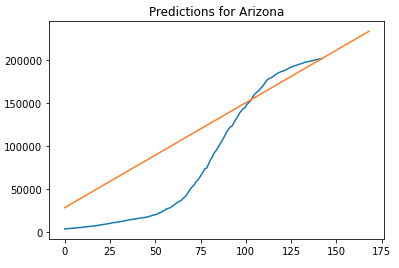
\includegraphics[width=\linewidth]{figures/7-linear-reg.png}
  \caption{Example of Linear Regression: $x$ is the numbers of days past our start date of April 1st, $y$ is the fitted line of confirmed cases for Arizona}
  \label{fig:linreg}
\end{figure}
\subsection{Polynomial Fitting}
To try and mimic the exponential increase that linear regression couldn't do, we chose to try a polynomial fitting approach. Polynomial fitting tries to best fit a line through our data points of degree N. So our hope is that the line continuing past our training data would better reflect the trend a particular state is showing. We used the scikit-learn package to transform our input to work with the degree N we want to fit\cite{scikit-learn}. This approach worked great at fitting our training data points. It also did a very good job at predicting the next few days for many states. We got best results with fitting a line of degree 3 and 5. We ended up deciding we would not go forward with it. We decided this because when it tries to fit the training data, the trend a few days after the end can either shoot upwards exponentially or begin to dip downward, where the number of predicted cases or deaths is actually lower than the previous day. We see this happening in Figure \ref{fig:polyfit} for the state of Arizona with a degree of 3. We thought we could mitigate this by predicting a few days ahead and then refitting until we had our full prediction. The big downfall of this approach is that it would compound any error we produced with our predictions to every other prediction made afterwards.
\begin{figure}
  \centering
  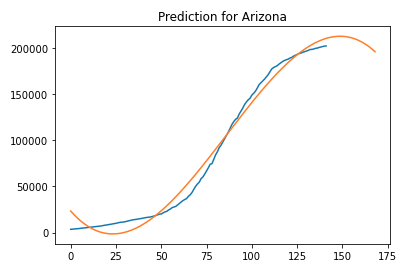
\includegraphics[width=\linewidth]{figures/7-poly-fit.png}
  \caption{Example of Polynomial Fitting: $x$ is the numbers of days past our start date of April 1st, $y$ is the fitted line of confirmed cases for Arizona}
  \label{fig:polyfit}
\end{figure}

\subsection{ARIMA}
Given the issue of producing predictions of confirmed cases and deaths without
having access to the values of the other features we would want to include in 
our model for the predicting time period. It was clear that time series algorithms
would be the best class of models for our data. The first model tried was the
Autoregressive (AR) model. The AR model uses a linear combination of previous
time steps to predict the future time steps. The equation for this model is \cite{forecasting},
\begin{equation}
 y_t = c + \phi_1 y_{t-1} + \phi_2 y_{t-2} + ... + \phi_p y_{t-p} + \epsilon_t 
\end{equation}
Where $y_t$ denotes the number of cases at time $t$, $\phi_j$ are the learned weights,
 $\epsilon_t$ is white noise and $c$ is a bias term. In this case we are looking at the last $p$ time days
for prediction, we denote this as an AR(p) model. 

To implement the model we use the 'AutoReg' module from the statsmodels package \cite{statsmodels}
and trained a unique AR model for each state. Since this model
was mainly explored during round 1, we used the data from the 2nd of August 2020 to the 31st of August 2020
as validation data. From this validation data we tuned $p$ to get the lowest overall mape for confirmed cases and deaths.
This led to an optimal $p$ of 3, however, our MAPE was still very high at $11.3$. What we saw in the model was that our
confirmed cases diverged significantly from the true values as time went on. When the AR model predicts future unseen values,
we have shown that the model must use previous time steps to predict the current one. Hence when looking at unseen data, 
the model will use previously predicted values to predict future values. This leads to a compounding of error and thus 
results in a diverging relationship between the true values and the predicted ones as can be seen in figure \ref{fig:AR}.
\begin{figure}
  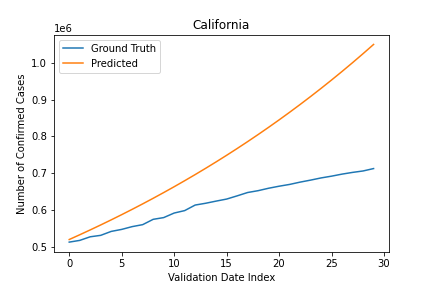
\includegraphics[width=\linewidth]{./figures/Section2_AR_Cali_Conf.png}
  \caption{Confirmed Cases in California predicted using AR}
  \label{fig:AR}
\end{figure} 
Our final round 1 MAPE using AR was $4.12$
The issue with our implementation of the model is that we did not enforce the stationarity of the data which 
is a prerequisite for the model. A stationary time series is one whose properties do not depend on the time at 
which the series is observed \cite{forecasting}.
This therefore shows AR's difficulty in accounting for the trend since stationary
data is devoid of one. Therefore we needed a model that was able to account for data with a trend. This is why we chose to 
explore the Autoregressive Integrated Moving Average (ARIMA) model. The Moving Average (MA) portion of ARIMA states that 
future time steps are predicted as a linear combination of previous forecast errors. The equation for this model is \cite{forecasting},
\begin{equation}
y_t = c + \sum_{i=1}^{q} \theta_i \epsilon_{t-i}
\end{equation} 
Where $\theta_i$ are the learned weights, $c$ is the bias term and $\epsilon_i$ are the white noise error terms that are 
seen in equation 1. Since we look at the last $q$ time steps, this is known as a MA(q) model.
Hence, a combination of the AR model and the MA model will reduce the compounding error problem from before since we
take the forecast errors into account. However both AR and MA models require data to be stationary which as shown before is not
the case. A way to make data stationary is by looking at the difference of contiguous time series values $y'_t = y_t - y_{t-1}$
as opposed to the values themselves. This process of differencing can be done multiple times if the initial differencing does
not yield a stationary time series.

Therefore, the ARIMA model incorporates differencing to give the forecasting equation \cite{forecasting},
\begin{equation}
  y'_t = c + \sum_{i = 1}^{p} \phi_i y'_{t-i} + \sum_{j=1}^{q} \theta_j \epsilon_{t-j} + \epsilon_t
\end{equation}
Which we see is a combination of equations 1 and 2 but on differenced values. Thus the $\epsilon_j$ are white noise errors for
$y'_j$ not the original time series $y_j$. As we mentioned, differencing can occur many times until stationarity is enforced,
we let the the number of time the data is differenced be denoted as $d$ the degree of differencing. Furthermore, we are
already aware of the parameters $p$ and $q$ from the respective AR and MA models. Hence we denote the above equation as an
ARIMA(p,d,q) model. 

\begin{figure}
  \centering
  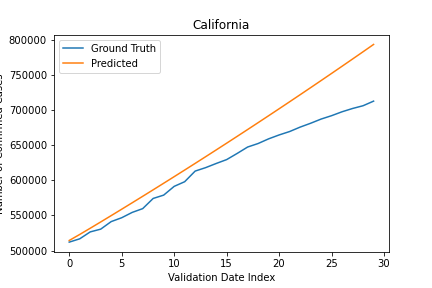
\includegraphics[width=\linewidth]{figures/Section2_ARIMA_Cali_Conf.png}
  \caption{Confirmed Cases in California predicted using ARIMA}
  \label{fig:ARIMA}
\end{figure}

From figure \ref{fig:ARIMA}, we see that the amount of divergence between predicted and actual values is much smaller due to including
a moving average and inducing stationarity.


To implement this model, we used the ARIMA module from the statsmodels package \cite{statsmodels}. There are, however, many
ways to find the optimal $p,d,q$ values. Initially we thought that since our metric of evaluation is MAPE, we could optimize
these parameters with respect to a validation MAPE and use those parameters to predict the future cases and deaths for a 
particular state. To do this, a simple grid search was done where $p,d,q$ values ranged from $1$ to $10$ and the tuple with the
lowest validation MAPE for that state was chosen. Initially we chose a validation size of 30 days. This yielded a final round 1 MAPE of $3.44$.
Although this was better than the AR model, it was still below the baseline MAPE. In addition, we saw an increased number 
of stationarity and convergence errors with our optimized set of tuples for certain states. In these cases, we had to resort to
using our naive AR implementation as backup. This indicated that our tuple was not fully capturing the trends in our data
by being optimizing for 30 days prior. 

Hence we chose to reduce our validation size to 7 days instead to see if having a larger amount of data and using a more
recent validation set would lead to a more representative optimal $p,d,q$ tuple. This was indeed the case as we were able to
get a round 1 MAPE of 2.96. We still ran into the stationarity and convergence errors and did have to use AR as a backup.
In this vein, we reduced the validaiton size further to only 3 days but this led to a MAPE of 4.71 indicating that we overfit
our validation data. 

The auto arima module from the pmdarima package \cite{pmdarima} uses a grid search similar to before to find the optimal
tuple. However, auto arima uses statistically rigorous stationarity tests (such as Augmented Dickey Fuller) to find 
the optimal order of differencing $d$ after which the optimal $p,q$ are found by minimizing the Akaike Information Criterion (AIC).
AIC is a measure of the quality of a model, it measures the likelihood of a model to predict future values \cite{AIC}. The equation
to calculate AIC is given by \cite{AIC},
\begin{equation}
  AIC  = -2 \cdot \ln(L) + 2k
\end{equation} 
Where $L$ is the likelihood of the model, and $k$ is the number of estimated parameters. A model with a lower AIC value
indicates a model of better quality. Optimizing by MAPE on a validation set runs the risk of being overfit to the validation
set as seen when we reduced our validation size to 3 days. Hence when looking a generalizable models for our round 2 submission,
it was important that we did not overfit to our current data. By using a measure that is trained insample and does not depend
on a validation set, the generalizability of the model increases. By optimzing for AIC we did get a lower MAPE than our previous
models so this was chosen as the optimization criteria when a state is trained using this method.


\subsection{HOLT}
Previously, our ARIMA and AR models used a linear combination of previous days to predict future days as well as include an 
order of differencing to induce stationarity. The linear combination in equation 3 implies that the learned $\phi$ and $\theta$
weights has the same degree of importance to predicting $y_t$ since all the weights are of degree 1. This means that for 
the ARIMA model each day has as similar degree of importance to the output. Obviously the magintude of the coefficients will
determine which days are more important than others but since they are all a linear combination their degree of importance is
nonetheless the same. In addition, by enforcing stationarity of the time series, we are intentionally ignoring any trend pattern
which leads to a large loss of information regarding covid cases since the plateaus and exponential growth of deaths and 
confirmed cases are meaningful in predicting future values.

The Holt linear trend method, which shall be referrred to as Holt, is capable of working with time series models with trend
as well as placing greater emphasis on more recent days as opposed to days further removed. From \ref{fig:ARIMA} we can see
that ARIMA cannot predict the plateau of cases further out from the model. Hence by focusing on more recent days,
it could be that local trends such as local plateauing or exponential growth can be better approximated. The Holt equations
are a set of three equations for each time step. The trend equation \cite{forecasting} is given by
\begin{equation}
  b_t = \beta^*(l_t - l_{t-1}) + (1-\beta^*)b_{t-1}
\end{equation}
Where $b_t$ is an estimate of the slope at time $t$, $0 \leq \beta^* \leq 1$ is a smoothing parameter for the trend and 
$l_t$ is an estimate of the level at $t$. To calculate the level \cite{forecasting}, we have
\begin{equation}
  l_t = \alpha y_t + (1 - \alpha)(l_{t-1} + b_{t-1})
\end{equation}
Where $0 \leq \alpha \leq 1$ is a smoothing parameter for the level 
Lastly, to forecast the value \cite{forecasting} we have that
\begin{equation}
  y_{t+h|t} = l_t + hb_t
\end{equation}
We place less emphasis on previous days since if we want to caluclate $y_{t+1|t}$ we need the level and trend estimations of
timestep $t$ which allows for a better understanding of the local trend at that time. Furthermore, unlike ARIMA when predicting
future values, we do not use previously predicted values to predict future ones. Rather, once the final level $(l)$ and trend $(b)$ values
are calculated , future time steps are a linear combination of that level and trend value $(l + hb)$ where $h$ denotes how far ahead
the forecast must predict. Therefore, unlike AR and to an extent ARIMA, we remove the compound error issue and we do not need to introduce
a moving average error equation to mitigate the compounded errors. 

In terms of implementation, we used the Holt module from the statsmodels package \cite{statsmodels}. Using an internal optimization process,
the ideal values of $\alpha, \beta^*, l_0, b_0$ are calculated after which the model calculates the remaining $l_t$ and $b_t$ values
and forecasts the predicted time series for cases and deaths per state. Implemented in a homogenous manner, i.e. the same model applied 
to all states, this model was our best peforming one, giving a round 1 MAPE of $2.289$. 

\begin{figure}
  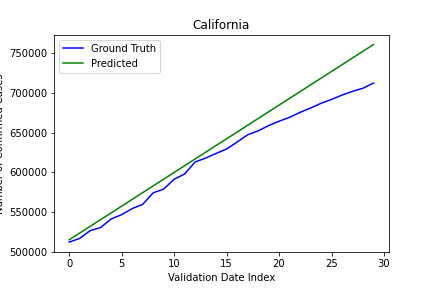
\includegraphics[width=\linewidth]{figures/HOLT_Cali_Conf.png}
  \caption{Confirmed Cases in California predicted using Holt Winters Linear Trend Method}
  \label{fig:HOLT}
\end{figure}
From \ref{fig:HOLT} we see that our forecast is a line, which is a direct result of equation 7 and that the line is closer to the actual number 
of confirmed cases than ARIMA. Therefore, the approximation of a local trend using the latest $l_t$ and $b_t$ values was indeed better than 
linearly weighting a certain number of previous time steps for California. While the lower MAPE indicates that Holt is a better model overall,
for certain states, Holt performs much worse than linear regression or ARIMA. When the states have a sudden increase or flattening of trend,
for example in Wyoming, Holt does a bad job of giving a generally accurate forecast since the local approximations are often not indicative of 
the evolution of cases and deaths in that state. Again, due to the local approximation issue, states who spiked in cases or deaths after the
training set were also not accurately forecasted.
\subsection{Exponential Smoothing}
\subsection{Long Short Term Memory Neural Networks}

Neural networks are shown to be incredibly malleable since there is a plentiful
amount of hyperparameters to tune and to create ranging from the type of
activation function to the architecture of the network. For sequential data
specifically, recurrent neural networks or RNNs work well mostly because it
allows previous outputs to be used as inputs while having hidden states.  
In the context of time series prediction and the task at hand, RNNs work well
since it can utilize previous timestamped or predicted data to predict other
output data. Inside each layer and node are specific functions that manipulate
the inputs known as gates.

\begin{figure}
  \centering
  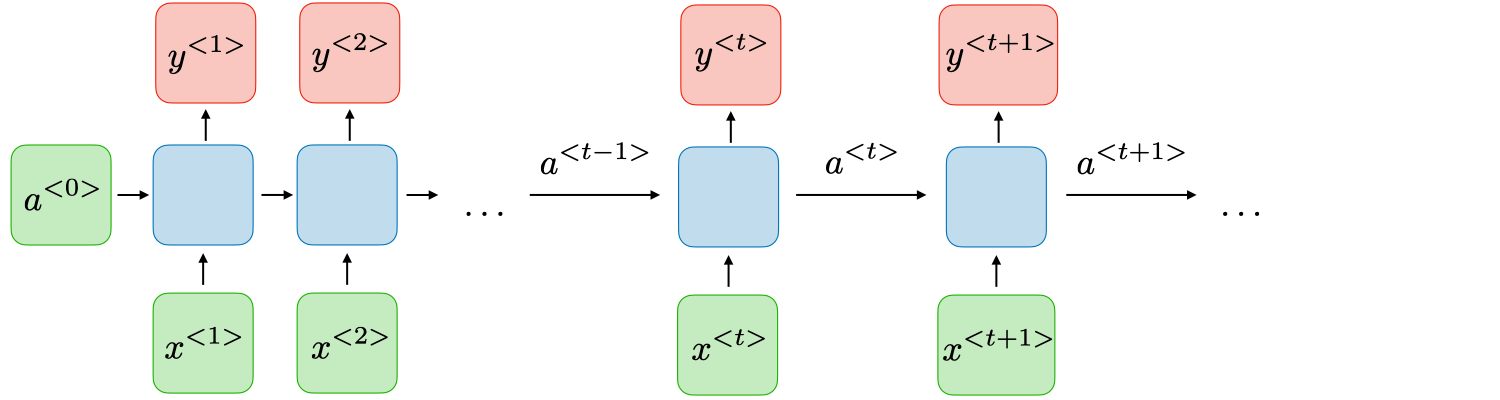
\includegraphics[width=\linewidth]{figures/architecture-rnn-ltr.png}
  \caption{Example of RNN: $x$ is the input, $y$ is the output, the middle blue
  cells are a part of the hidden layer}
  \label{fig:rnn}
\end{figure}

Within the context of RNNs, there is a set of specific RNNs called Long Short
Term Memory Neural Networks or LSTM for short. What is specific of the LSTM is
that it utilizes a specific set of 3 gates: an update, output, relvance, and
forget gate \cite{LSTMlecture}. This allows LSTM neural networks to regulate
the flow of information and decide how much past data affects the current
prediction, generalizing better for time-series specific tasks.

Given this context, and before using this method as our main modeling choice,
we needed to validate this method. Using the PyTorch neural network framework
\cite{Pytorch}, a simple RNN neural network of 1 layer with 50 LSTM nodes was
tested on a subset of the round 1 data. 

\begin{figure}
  \centering
  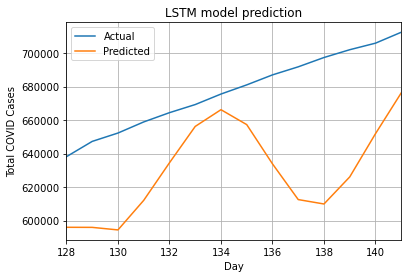
\includegraphics[width=\linewidth]{figures/LSTMPytorch.png}
  \caption{LSTM predictions on data pertaining to California}
  \label{fig:LSTM_trial}
\end{figure} 

The experimentation procedure would use the confirmed case and death count data
from April 12th to August 17th for the state of California and then validating
the MAPE over a period of 14 days, August 18th to August 31st. The neural
network will be trained over a varied amount of epochs and learning rates. 
Attached on Figure  \ref{fig:LSTM_trial} is an example trial run of our
prediction using the PyTorch neural network. The MAPE on this was around $6.93$
which was much higher than the other methods.

Given the lackluster results, amount of time required to tune each parameter,
and the non-deterministic nature of neural networks, the use of LSTM neural
networks was not really explored deeply with the rest of the dataset.

\subsection{Other Methods}

In addition to the specific models, we also tested some other time-series
specific methods using the AtsPy software library \cite{atspy}. This software
package contains Python implementations of the Prophet, Gluonts, and TBATS methods 
that were easily to be trained using the data that had been split into training
and validation datasets.

Prophet is a procedure used by the Facebook Data Science team for their time 
series forecasting \cite{Prophet}. It was very complicated and convoluted to 
use and the MAPE results that it gave on the validation set was not feasible 
for us to use as our main method of forecasting.

Gluonts is an RNN based framework for time series forecasting \cite{Gluonts}. It uses
probabilistic modeling in order to predict and forecast future time-series
data. Again, the MAPE results were very poor and its complexit was not worth
the amount of time that we had.

TBATS is a method that uses something called a Box-Cox transformations to 
forecast future time series data points \cite{TBATS}. The MAPE results it yielded from
a simple validation on the last week of data were too  poor to necessitate 
further research and its complexity further hindered it.


\subsection{Conclusions}

Methods such as LSTMs and Prophet were too complex for our use case and time
duration. Given the amount of time we had and the necessary work needed, we
could not optimize these methods and their hyperparameters for our situation
and thus we disregarded using these methods for the final code submission.
Our best performing metrics were simple univariate time series algorithms such
as HOLT, linear regression, and ARIMA. 

Of these three models, HOLT model typically gives us the lowest overall MAPE.
However, it consistently underperforms on certain states. Linear Regression and
ARIMA may yield significantly better results for these "problem states".
However, it is not always easy to tell which states are going to cause problems
with the HOLT model -- performance varies significantly based on the shape of
the latest batch of test data. This heterogeneity makes it very difficult to
pick a "favored model" for our time series predictions. 

However, not all of our conclusions are subject to this variance. While model
\emph{performance} varied significantly based on the target state, the "optimal
hyperparameters" used to train a given models do not change significantly on a
state-by-state basis. By performing grid search on each model's
hyperparameters, we developed a group of parameterized models that handle
general state data reasonably well. 



\section{Final Model Design}

The pros and cons (as well as the relative efficacy) of each model have already
been discussed. Faced with such a diversity of model performance, we opted to
use a hybrid model for our overall submission. 

Both rounds used a univariate data model (ie. trained only on the number of
deaths or confirmed cases), and were trained state-by-state (ie. a new model
was trained on each state's data; this model's predictions became our
predictions for the given state). An overview of our methodology follows. 

\subsection{Round 1}

Our Round 1 modelling method used a comparatively straightfoward "hybrid"
approach. We split our training data by state, then manually ran HOLT and
linear regression models on the state's data (using the last few weeks as
validation data). We noted which models gave us a lower MAPE for which states,
and hardcoded these $(state, model)$ associations into our script, assuming
that these trends would hold. For example, linear regression usually
outperformed HOLT for predicting deaths in the state of Montana; we accordingly
instructed the computer to always use linear regression when predicting
Montana's deaths. 

However, this mapping wasn't sufficient. 
Model performance is a function of the total amount of data given to the model;
for time series data, this includes our start date. Linear regression, for
example, may perform better when given only the last 2 weeks of data (to
understand why, consider the effect of step size on linear gradient descent
when trying to fit an exponential curve). 
Every model was thus given a \emph{start date} parameter, which was defined as
the date of the oldest training datapoint that the model received. 
For Round 1, we set this parameter manually on a state-by-state basis by
hardcoding it into our script. 

After building up this database of optimal start dates and optimal models, we
wrote a Python script that trained the given models (using \cite{scikit-learn}'s
\texttt{linear\_model.LinearRegression} class and the \texttt{Holt} module from
the \cite{statsmodels} library). We then used the library routines to give us
time series predictions for the required number of days. 

\subsection{Round 2}

After completing Round 1 of the project, we began to realize that manually
cherry-picking an appropriate model for each state was not scalable. 

We had no way to test quick adjustments to our hyperparameters, which made
manual optimization tedious. In addition, we had no way of effectively
determining the best \emph{start\_date} for a given model on a given state. 
We opted to shift towards an automated approach towards model selection. 
Otherwise, our methodology remained the same as in Round 1, where we would test
multiple \emph{start\_dates} and validate them over a small validation set segregated
from the original training data.

Suppose that we are given $n$ days of training data, and are tasked with
predicting $m$ days in the future. 

\begin{figure}
  \centering
  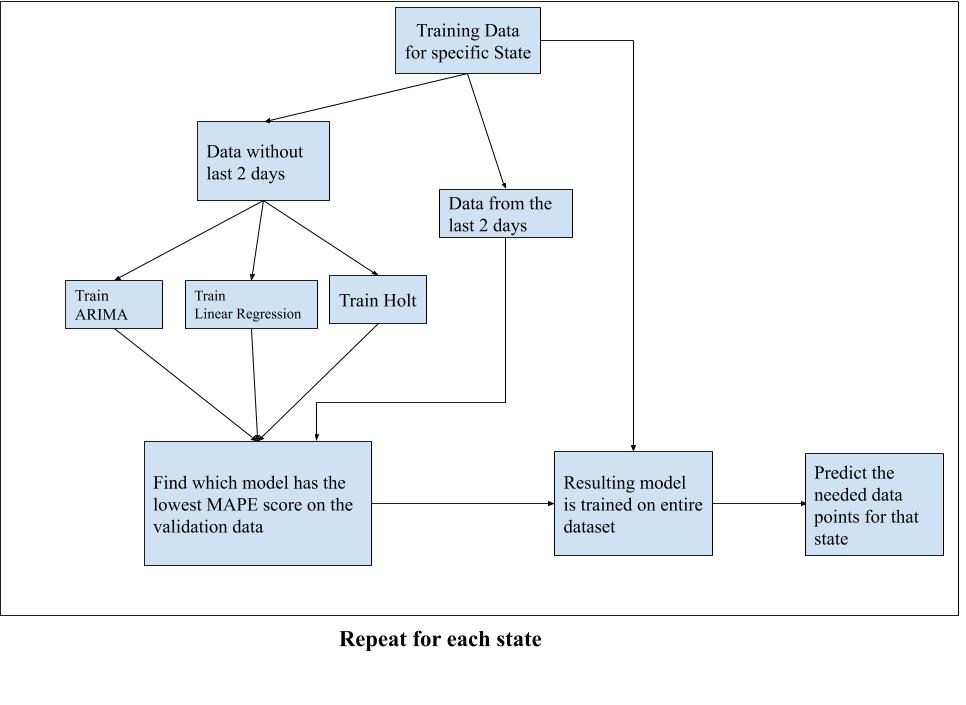
\includegraphics[width=\linewidth]{figures/Final_model.jpg}
  \caption{An flowchart of what our Round 2 model does}
  \label{fig:model_final}
\end{figure}

First, we segregate the data again. Given $n$ days of training data, our model
uses the first $n-2$ days to train on (we'll call this set $T$) and the last
$2$ days as a validation dataset (we'll call this subdivision $V$). We then
train Linear Regression, HOLT, and ARIMA models on $T$, predicting $m+2$ days
into the future. We take the first $2$ days of these predictions, and calculate
the MAPE using $V$. After comparing the MAPEs of each model on $V$, we choose
the model that gives us the lowest MAPE for that particular state, and return
the remaining $m$ predicted days. An example iteration can be seen in the 
Figure \ref{fig:model_final} which shows a visual flowchart of what is being done
for each state.

After observing our hybrid model, we noted two trends: 
\begin{itemize}
\item 
Splitting our data into $T$ and $V$ caused some of our models to
underperform. This is because they effectively had to predict $m+2$ days into
the future as opposed to $m$ days (the first two days, of course, were used for
our validation and model selection). This underperformance wasn't uniform;
HOLT tended to give us relatively accurate predictions, while linear regression
tended to underpredict the number of deaths. 
\item
Different models often give similar MAPEs when evaluated on $V$. 
\end{itemize}

Given these two points, we added an $\epsilon$ "margin" term to our final
implementation. If two models perform comparatively (ie. within $\epsilon$ MAPE
of each other) on $V$, then our framework prefers the model that "generalizes
better" as per our heuristic observations. For example, if linear regression
and HOLT both get an MAPE of $8.675309 \pm (\epsilon = 0.001)$, our framework
will use HOLT to predict the values for the state. Our framework prefers HOLT
to linear regression if the MAPEs are similar, but doesn't put ARIMA into this
"margin" framework (ie. if ARIMA yields the lowest MAPE, ARIMA will always be
chosen). The addition of this $\epsilon$ parameter yielded an experimental 
MAPE improvement of around 0.05. 

\section{Conclusion}

\section{Task Distribution Form}

We'll be referring to group members by their initials: Hamlin Liu is HL; Juan
Estrada is JE; Justin Yi is JY; Shriniket Buche is SB; Yash Lala is YL. 

\begin{table}[h!]
    \centering
    \begin{tabular}{|c|c|}
        \hline
         Task & People  \\
         \hline \hline
         Exploratory Data Analysis & HL, JE, JY, SB, YL \\
         \hline
         Normalization code & JY \\
         \hline
         Linear Regression testing & JE \\
         \hline
         ARIMA testing & SB \\
         \hline
         AR testing & SB \\
         \hline
         HOLT testing & JE, SB \\
         \hline
         LSTM and BiLSTM model testing & HL, SB  \\
         \hline
         VAR model testing & JY, SB \\
         \hline
         Gluonts, Prophet, and BATS model testing & SB \\
         \hline
         Data Clustering & JY, YL \\
         \hline
         Data Interpolation & YL \\
         \hline
         Midterm Report Writing & HL, JE, JY, SB, YL \\
         \hline
         Midterm Report Formatting & HL, YL \\
         \hline
         Scraping for new data & HL \\
         \hline
         Kaggle Submissions & JE, SB \\
         \hline
         Round 1 code & HL, JE \\
         \hline
         Round 2 code & HL, JY, YL \\
         \hline
         Final Report writing & HL, JE, JY, SB, YL \\
         \hline
    \end{tabular}
\end{table}


\bibliographystyle{ACM-Reference-Format}
\bibliography{report}

\end{document}
\endinput
